\documentclass[aspectratio=169]{beamer}
\usetheme{Madrid}
\usecolortheme{default}

\usepackage{booktabs}
\usepackage{graphicx}
\usepackage{amsmath}

\title{Optimus Primal --- Gait Optimization}
\subtitle{From Hand-Tuned Crawl to Learned Locomotion}
\author{Darien Parris}
\date{\today}

\begin{document}

\begin{frame}
\titlepage
\end{frame}

% ------------------------------------------------------------------
% Slide 1: Problem
% ------------------------------------------------------------------
\begin{frame}{Problem}
\begin{itemize}
    \item \textbf{Slow iteration loop} --- each hand-tuned gait takes minutes to test on hardware; no way to explore the full parameter space
    \item \textbf{Stride length hit a stability ceiling} --- longer strides toppled the robot; couldn't find the right weight-shift timing by hand
    \item \textbf{Discrete hand-scripted phases don't generalize} --- moving to simulation lets the robot optimize against \emph{intrinsic} goals (keep the frame parallel to the ground) rather than fixed motor sequences
\end{itemize}
\end{frame}

% ------------------------------------------------------------------
% Slide 2: Digital Twin
% ------------------------------------------------------------------
\begin{frame}{Digital Twin --- URDF to MuJoCo}
\begin{itemize}
    \item Built from the same \texttt{optimus\_primal.urdf} the real robot uses --- same link geometry, joint limits, effort caps
    \item 8 actuated joints (4 hips + 4 knees) driven by \textbf{position servos} ($k_p{=}2.5$, $k_v{=}0.05$, initial guess; bench-measured later --- see slide 13)
    \item Free joint on \texttt{base\_link} --- physics decides what happens; no kinematic cheating
    \item Floor: flat plane with friction $\mu{=}1.0$ (rubber/TPU-sock approximation)
    \item \textbf{Caveat:} CAD wasn't modeled at the origin, so STL meshes render detached. Collision geometry is correct; visual hidden via \texttt{discardvisual}. Cosmetic only --- physics unaffected.
\end{itemize}
% \includegraphics[width=0.4\textwidth]{sim_screenshot.png} % add screenshot
\end{frame}

% ------------------------------------------------------------------
% Slide 3: Search Space
% ------------------------------------------------------------------
\begin{frame}{Search Space --- 105 Parameters}
\begin{itemize}
    \item Gait \textbf{structure is fixed}: 13 phases in a crawl cycle\\
          \texttt{start} $\to$ \texttt{\{shift, swing, plant\}} $\times$ \texttt{\{FR, RL, FL, RR\}}\\
          Optimizer tunes the \textbf{angles at each phase}, not the sequencing
    \item \textbf{104 joint-angle params:} 13 phases $\times$ 4 legs $\times$ 2 joints (hip + knee), in degrees
    \item \textbf{+1 phase-time param:} seconds between phases --- controls gait cadence
\end{itemize}

\vspace{0.3em}
\begin{tabular}{lll}
    \toprule
    Parameter & Lower Bound & Upper Bound \\
    \midrule
    Hip angle       & $5^\circ$   & $55^\circ$ \\
    Knee angle      & $-100^\circ$ & $-25^\circ$ \\
    Phase time      & 0.15\,s     & 1.2\,s \\
    \bottomrule
\end{tabular}

\vspace{0.3em}
\begin{itemize}
    \item \textbf{Seeded from the hand-tuned gait} --- generation~1 already walks
    \item \textbf{Sim-to-real is a parameter copy} --- same degree convention as the robot's motor controller; winning JSON loads directly onto hardware
\end{itemize}
\end{frame}

% ------------------------------------------------------------------
% Slide 4: Algorithm --- CMA-ES
% ------------------------------------------------------------------
\begin{frame}{Algorithm --- CMA-ES}
\textbf{Covariance Matrix Adaptation Evolution Strategy}\\[0.3em]
Gradient-free, population-based optimizer --- the standard for robot gait tuning.

\vspace{0.5em}
\textbf{Each generation:}
\begin{enumerate}
    \item Sample 48 candidate gaits from a multivariate Gaussian $\mathcal{N}(\mathbf{m},\,\sigma^2 \mathbf{C})$
    \item Evaluate every candidate in MuJoCo --- in parallel across CPU cores
    \item Rank by reward, keep the top half
    \item Update the distribution:
    \begin{itemize}
        \item \textbf{Mean} $\mathbf{m}$ moves toward the winning region
        \item \textbf{Covariance} $\mathbf{C}$ stretches along directions that produced good solutions
        \item \textbf{Step size} $\sigma$ grows or shrinks based on progress
    \end{itemize}
\end{enumerate}

\vspace{0.5em}
\textbf{Engineering:} popsize\,=\,48, $\sigma_0$\,=\,5.0, auto-restart on 15-gen stall,\\
parallel evaluation ($\sim$7$\times$ speedup on 8-core Mac), checkpoint every generation.
\end{frame}

% ------------------------------------------------------------------
% Slide 5: Reward Function
% ------------------------------------------------------------------
\begin{frame}{Reward Function}
\textbf{Shaped iteratively through failure.}

\vspace{0.3em}
\small
\begin{tabular}{llr}
    \toprule
    Component & Purpose & Weight \\
    \midrule
    Forward distance        & Primary goal          & $+100$/m \\
    Phases completed        & Survival bonus        & $+0.5$/phase \\
    Mean body height        & Don't collapse        & $+5$ \\
    Backward distance       & Wrong direction       & $-200$/m \\
    Mean pitch$^2$          & Stay level (F/B)      & $-30$ \\
    Mean roll$^2$           & Stay level (L/R)      & $-40$ \\
    Peak pitch/roll$^2$     & No big momentary tilts & $-8$ each \\
    \textbf{Mean nose-down}$^2$ & \textbf{Don't flop forward} & $\mathbf{-200}$ \\
    \textbf{Peak nose-down}$^2$ & \textbf{Not even once}      & $\mathbf{-60}$ \\
    Mean pitch-rate$^2$     & No floppy motions     & $-2$ \\
    \bottomrule
\end{tabular}
\normalsize

\vspace{0.3em}
\textbf{Hard terminations:} body height $<8$\,cm, any tilt $>30^\circ$, nose-down $>27^\circ$.
\end{frame}

% ------------------------------------------------------------------
% Slide 5b: Reward Iteration Story
% ------------------------------------------------------------------
\begin{frame}{Reward Function --- Iteration Story}
\textbf{Each version was shaped by watching what the optimizer exploited.}

\vspace{0.5em}
\begin{description}
    \item[v1 --- Distance only] Robot learned to collapse onto its shins and scoot forward.\\
        Technically moved. Not a gait.
    \item[v2 --- Symmetric tilt penalty] Tightened fall threshold from $45^\circ$ to $30^\circ$.\\
        Better balance, but still toppled forward during swing phases.
    \item[v3 --- Directional nose-down + pitch-rate] Targets the specific forward-flop failure mode without penalizing backward lean (useful for weight shifting).
\end{description}

\vspace{0.5em}
\emph{The reward function is as much the product of learning as the gait itself.}
\end{frame}

% ------------------------------------------------------------------
% Slide 6: Results --- Seed Comparison
% ------------------------------------------------------------------
\begin{frame}{Results --- Does the Starting Point Matter?}
Three CMA-ES runs, same reward function, different seeds:

\vspace{0.3em}
\begin{description}
    \item[Hand-tuned gait] Seeded from the manually-tuned \texttt{stance.py} crawl
    \item[Random] Uniform random within bounds
    \item[Neutral standing] Every phase pinned to the standing pose (no motion)
\end{description}

\vspace{0.5em}
% \includegraphics[width=0.7\textwidth]{convergence_comparison.png}

\vspace{0.3em}
\textbf{Takeaway:} Seeding from a human-tuned gait gives a massive head start --- generation~1 is already walking, so the optimizer spends its budget \emph{refining} instead of \emph{discovering}.
\end{frame}

% ------------------------------------------------------------------
% Slide 6b: Results --- Algorithm Comparison
% ------------------------------------------------------------------
\begin{frame}{Results --- Algorithm Comparison}
Same reward function, same seed, different optimization algorithms:

\vspace{0.3em}
\begin{description}
    \item[CMA-ES] Population-based, learns covariance structure of the search space
    \item[Differential Evolution] Population-based, mutates by combining existing solutions
    \item[Random Search] Uniform sampling baseline --- ``does optimization even help?''
\end{description}

\vspace{0.5em}
% \includegraphics[width=0.7\textwidth]{convergence_algo_comparison.png}

\vspace{0.3em}
% Add key finding here once data is available
\end{frame}

% ------------------------------------------------------------------
% Slide 7: Limitation
% ------------------------------------------------------------------
\begin{frame}{Limitation --- Open-Loop Control}
\textbf{CMA-ES found the best choreography. But it's still a choreography.}

\vspace{0.5em}
\begin{itemize}
    \item Output is a \textbf{fixed lookup table}: 13 phases, 8 angles each, played back identically every stride
    \item No sensors, no feedback, no ability to react
    \item Works in sim (perfect flat floor) but struggles on real hardware
\end{itemize}

\vspace{0.5em}
\begin{tabular}{lll}
    \toprule
    & CMA-ES (current) & What we need \\
    \midrule
    Output              & 105 fixed numbers       & A function that reacts \\
    Sensors at runtime  & None --- blind playback  & IMU, joint positions \\
    Adapts to disturbance & No                     & Yes \\
    What it learned     & ``The best script''      & ``How to walk'' \\
    \bottomrule
\end{tabular}
\end{frame}

% ------------------------------------------------------------------
% Slide 8: Next --- RL
% ------------------------------------------------------------------
\begin{frame}{Next --- Reinforcement Learning}
\textbf{Close the loop: from choreography to skill.}

\vspace{0.5em}
RL trains a neural network (a ``policy'') that takes sensor readings \emph{every timestep} and outputs motor commands:

\vspace{0.3em}
\centering
\texttt{observe} $\to$ \texttt{decide} $\to$ \texttt{act} $\to$ \texttt{observe} $\to$ \texttt{decide} $\to$ \texttt{act} $\to$ \ldots

\vspace{0.5em}
\raggedright
\textbf{What we reuse:}
\begin{itemize}
    \item The MuJoCo digital twin --- same sim
    \item The reward function --- same objectives, already well-shaped
    \item The CMA-ES gait --- baseline to beat, can seed the initial policy
\end{itemize}

\textbf{What's new:}
\begin{itemize}
    \item Observation space: IMU (pitch, roll, $\dot{\theta}$) + 8 joint positions + 8 joint velocities
    \item Algorithm: PPO (Proximal Policy Optimization)
    \item Output: a neural network, not a JSON of fixed angles
\end{itemize}

\vspace{0.3em}
\emph{CMA-ES found the best choreography for a perfect floor.\\
RL will learn to actually walk --- adjusting every step based on what the robot feels.}
\end{frame}

% ------------------------------------------------------------------
% Slide 9: PPO Reward Engineering Journey
% ------------------------------------------------------------------
\begin{frame}{PPO --- Reward Engineering Journey (v5--v34)}
\textbf{30+ reward variants. Learning the failure modes was the work.}

\vspace{0.5em}
\small
\begin{tabular}{lll}
    \toprule
    Era & What we tried & What broke \\
    \midrule
    v5--v14 & Distance + tilt + height + extension       & ``Reward-engineering ceiling'' --- combined~$\sim$13 \\
    v15--v18 & Stride-detection bonuses (\textbf{silent bug}) & Foot-name lookup returned --1; rewards never fired \\
    v20 & Post-fix recipe                                & Combined $\sim$42; new champion \\
    v23--v26 & Body-smoothness + foot-drift penalties    & Body smoothness helped (N=2, noisy) \\
    v27--v29 & Survival bonus, fall-penalty schedules    & Most regressed; high seed variance \\
    v30 & \textbf{Friction domain randomization}         & \emph{Best sim result, doesn't deploy} \\
    v31 & High kp ($k_p$=20) for deployable PD          & Policy never learned to walk \\
    v33--v34 & X-config + low-friction + moderate steps & Same actuator-gap, 70--82\% bang-bang \\
    \bottomrule
\end{tabular}
\normalsize

\vspace{0.5em}
\textbf{High-water marks:} v20 (combined~$\sim$42), v25\_scratch\_3M\_b (44.7), v26\_body\_smooth\_b (44.9).\\
\emph{Across 23 trials in 9 cohorts, within-cohort seed variance ($\pm$10--30) dominated between-cohort effects.}

\vspace{0.3em}
\centering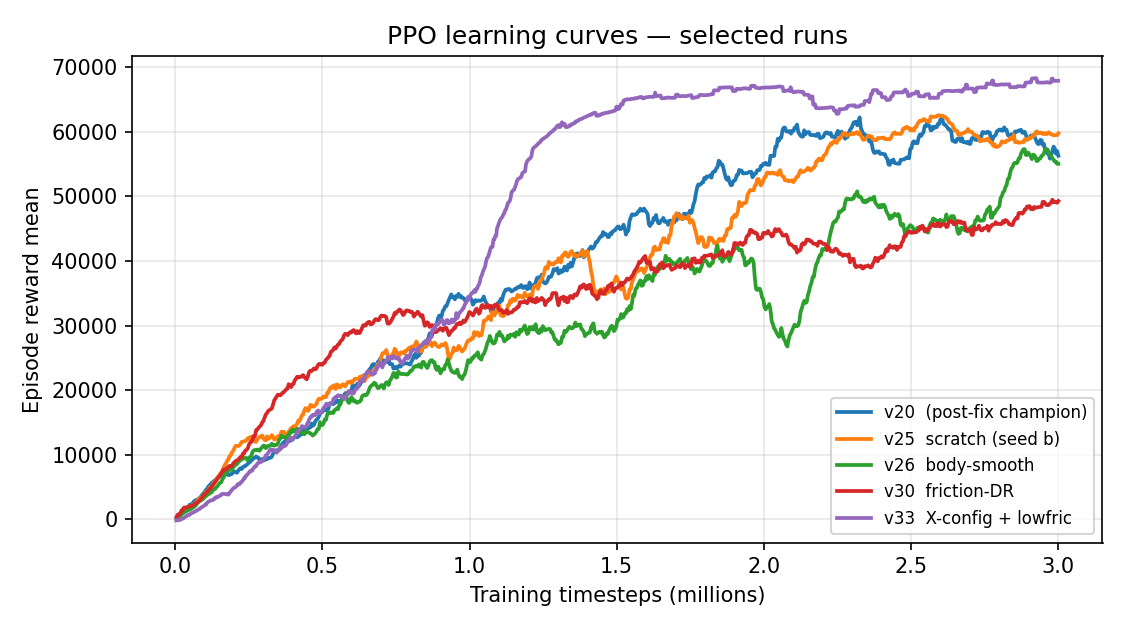
\includegraphics[width=0.78\textwidth]{ppo_learning_curves.png}
\end{frame}

% ------------------------------------------------------------------
% Slide 10: Friction Domain Randomization
% ------------------------------------------------------------------
\begin{frame}{Sim-to-Real --- Friction Domain Randomization (v30)}
\textbf{Real surfaces aren't sim-default ($\mu{=}1.0$). Trained three variants over $\mu \in [0.3, 1.0]$.}

\vspace{0.3em}
\small
\begin{tabular}{lcccc|c}
    \toprule
    & $\mu{=}1.0$ & $\mu{=}0.7$ & $\mu{=}0.5$ & $\mu{=}0.3$ & $\Delta(1.0\to0.3)$ \\
    \midrule
    \textbf{bodysmooth\_dr} & 50.5\,m & 56.4\,m & 54.0\,m & \textbf{53.9\,m} & \textbf{+7\%} \\
    v20\_dr               & \textbf{61.2\,m} & 56.5\,m & 51.5\,m & 49.4\,m & $-19$\% \\
    v6trig\_dr            & 35.1\,m & 37.1\,m & 35.1\,m & 39.6\,m & $+13\%$ \\
    \bottomrule
\end{tabular}
\normalsize

\vspace{0.5em}
\textbf{Finding:} \texttt{bodysmooth\_dr} is \emph{flat across the friction range} --- exactly what DR was supposed to produce. Pick for any low-friction deploy surface.

\vspace{0.5em}
\textit{But} --- preparing this for hardware uncovered the \textbf{actuator gap}, a sim-to-real failure mode unrelated to friction.
\end{frame}

% ------------------------------------------------------------------
% Slide 11: Actuator Gap (the surprise)
% ------------------------------------------------------------------
\begin{frame}{The Actuator Gap --- Why PPO Doesn't Deploy}
\textbf{Setup:} Trying to load the v30 friction-DR champion onto hardware revealed something more fundamental than friction.

\vspace{0.5em}
\textbf{Diagnostic measurements:}
\begin{enumerate}
    \item \textbf{Bang-bang action saturation: 88\%}\\
        Almost every commanded joint target is at the action-space LOW or HIGH.
    \item \textbf{Joint qpos response oscillates hard}\\
        Under MuJoCo's PD ($k_p{=}2.5$, $k_v{=}0.05$), the joint slowly chases the bang-bang target. P95 $|\Delta q|/$step$~= 17^\circ$.
    \item \textbf{Open-loop replay test: 65.8\,m $\rightarrow$ 0.57\,m}\\
        Take the joint trajectory the body actually followed, feed it as the env's target sequence in a fresh deterministic rollout. The body doesn't walk anymore.
\end{enumerate}

\vspace{0.5em}
\textbf{Interpretation:} \emph{Walking lives in the bang-bang action stream interacting with the PD, not in the resulting joint trajectory.} PPO discovered the underdamped PD acts as a low-pass filter; saturated commands at the right phase produce useful body motion. Same trick can't reproduce on the LX-16A's trajectory generator.

\vspace{0.3em}
\textbf{Consequence:} CMA-ES gaits deploy because their slow phase times ($0.6$--$1.4$\,s) let the PD settle. PPO at 62.5\,Hz operates inside the PD's transient response --- which is sim-specific.
\end{frame}

% ------------------------------------------------------------------
% Slide 12: ANYmal X-config experiment
% ------------------------------------------------------------------
\begin{frame}{ANYmal X-Config --- Geometry Experiment}
\textbf{Hypothesis:} An X-stance (front knees forward, rear hips swept forward, all four feet under chassis) might be more stable to walk on than the mammalian default.

\vspace{0.5em}
% \includegraphics[width=0.45\textwidth]{xconfig_pose.png}
\begin{itemize}
    \item Hand-posed the robot kinesthetically; captured per-leg servo angles
    \item Built \texttt{optimus\_primal\_xconfig.urdf} with rear hip + rear knee axes flipped
    \item Hardware \texttt{--xconfig} flag mirrors the same flip in \texttt{leg\_abs}
    \item Visual sanity-check via \texttt{view\_xconfig.py} --- chassis stands level, four feet planted
\end{itemize}

\vspace{0.5em}
\textbf{X-config CMA:} climbed cleanly to \textbf{best $\approx +686$} by gen $\sim$300 ($\sim$84\% of the mammalian gen-2500 winner at $\frac{1}{5}$ the compute).

\vspace{0.2em}
\centering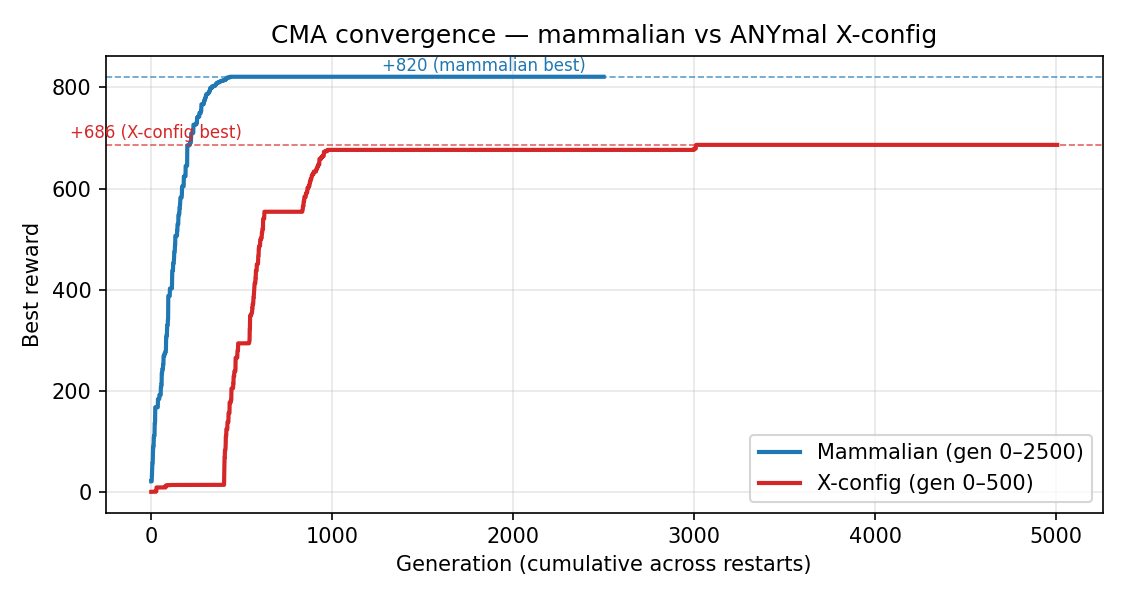
\includegraphics[width=0.85\textwidth]{convergence_xconfig.png}

\vspace{0.2em}
\raggedright\textbf{X-config PPO:} same actuator-gap. Geometry doesn't fix the bang-bang trap --- that's an actuator-model problem, not a geometry problem.
\end{frame}

% ------------------------------------------------------------------
% Slide 13: Bench Calibration of kp/kv
% ------------------------------------------------------------------
\begin{frame}{Closing the Sim-to-Real Loop --- Bench Calibration}
\textbf{Measure the actual LX-16A response, fit MuJoCo PD parameters to match.}

\vspace{0.3em}
\texttt{robot/motor\_step\_response.py} on the Pi:
\begin{enumerate}
    \item Step each of 8 servos $\pm 10^\circ$ from current position
    \item Sample \texttt{get\_physical\_angle()} at 50\,Hz for 300\,ms each direction
    \item Save the time-series as JSON
\end{enumerate}
\texttt{sim/fit\_pd\_from\_step\_response.py} on the Mac: sweeps MuJoCo $(k_p, k_v)$, finds best fit per servo.

\vspace{0.5em}
\textbf{Result:}
\small
\begin{tabular}{lccc}
    \toprule
    Joint type & $k_p$ & $k_v$ & RMSE \\
    \midrule
    Front hips         & 0.47 & 1.23 & 6.0$^\circ$ \\
    Rear hips          & 1.14 & 1.92 & 5.4$^\circ$ \\
    All knees          & 0.73 & 0.5--0.9 & 7.0$^\circ$ \\
    \midrule
    \textbf{Median}    & \textbf{0.73} & \textbf{0.87} & --- \\
    \bottomrule
\end{tabular}
\normalsize

\vspace{0.5em}
\textbf{Two conclusions:}
\begin{enumerate}
    \item Original $k_p{=}2.5$ was \emph{too stiff} --- sim was a faster actuator than reality.
    \item RMSE of $5$--$7^\circ$ on a $10^\circ$ step won't go away. \textbf{The LX-16A is a trajectory generator, not a PD.} No $(k_p, k_v)$ matches a constant-velocity ramp using exponential approach.
\end{enumerate}
\end{frame}

% ------------------------------------------------------------------
% Slide 14: Velocity-slew Actuator Fix
% ------------------------------------------------------------------
\begin{frame}{The Fix --- Velocity-Slew Actuator}
\textbf{Don't tune the gains. Change the actuator model.}

\vspace{0.5em}
Added \texttt{slew\_rate\_dps} parameter to \texttt{OptimusPrimalEnv.step()}: per-substep update to \texttt{data.ctrl} is clamped to \texttt{slew\_rate $\times$ dt} of change toward the policy's action. Emulates the LX-16A's internal constant-velocity trajectory generator at the actuator level.

\vspace{0.5em}
\textbf{Verified:} a bang-bang action stream now produces only $\sim 0.6^\circ$/env-step of joint motion at $125^\circ$/s slew rate (vs the unconstrained PD's $\pm 17^\circ$/step).

\vspace{0.5em}
\textbf{What this enables (untested at submission time):}
\begin{itemize}
    \item PPO action stream becomes the deployable trajectory --- each action is a position target the LX-16A interpolates to over the 16\,ms ctrl interval
    \item Bang-bang is impossible: the sim physically rate-limits the action stream before it ever reaches the PD
    \item Deployability gate: if \texttt{ppo\_actuator\_gap.py} reports saturation $<30\%$ AND replay ratio $>50\%$, the trace ports to hardware via \texttt{LX16A.move(angle, time=16)} calls
\end{itemize}

\vspace{0.3em}
\textbf{CMA gaits unaffected} --- they don't go through gym\_env, and their slow phase times already cleared the actuator gap.
\end{frame}

% ------------------------------------------------------------------
% Slide 15: Where We Land
% ------------------------------------------------------------------
\begin{frame}{Where We Land --- Submission Snapshot}
\textbf{What deploys to hardware today:}
\begin{itemize}
    \item \textbf{Mammalian CMA gait} (\texttt{best\_gait.json}, +821 reward, gen 2500)
    \item \textbf{X-config CMA gait} (\texttt{cma\_xconfig.json}, +680 reward, gen $\sim$300)
    \item Both load directly via \texttt{gait\_controller.py --gait <file>}
\end{itemize}

\vspace{0.5em}
\textbf{What we learned that the slides don't fully convey:}
\begin{itemize}
    \item Reward shaping is a search problem within the search problem
    \item Seed variance dominates ablation effects until you commit to 5+ seeds per cell
    \item Sim-to-real is not one gap, it's a stack: friction, then actuator-model, then sensor model
\end{itemize}

\vspace{0.5em}
\textbf{What's next, ready but unrun:}
\begin{itemize}
    \item PPO with \texttt{--slew-rate 125 --kp 20} --- the hypothesis is that the velocity-slew actuator removes the bang-bang exploit and makes PPO traces deployable
    \item Bench friction calibration (the same step-response idea, but for $\mu$)
\end{itemize}

\vspace{0.5em}
\centering\textit{Optimizing the gait was easy compared to learning what we were optimizing for.}
\end{frame}

\end{document}
